% 画网络图
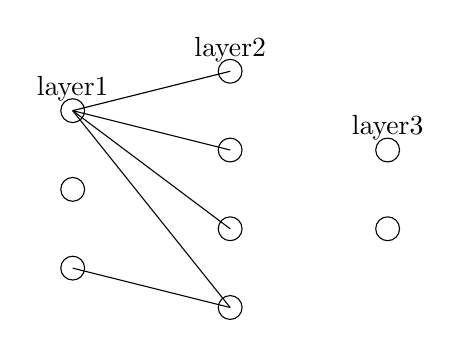
\begin{tikzpicture}
\coordinate (a1) at (0,0);
\coordinate (a2) at (0,-1);
\coordinate (a3) at (0,-2);
\coordinate (b1) at (2,0.5);
\coordinate (b2) at (2,-0.5);
\coordinate (b3) at (2,-1.5);
\coordinate (b4) at (2,-2.5);
\coordinate (c1) at (4,-0.5);
\coordinate (c2) at (4,-1.5);

\draw (a1) circle (1ex) node[above]{layer$1$};
\draw (a2) circle (1ex);
\draw (a3) circle (1ex);
\draw (b1) circle (1ex) node[above]{layer$2$};
\draw (b2) circle (1ex);
\draw (b3) circle (1ex);
\draw (b4) circle (1ex);
\draw (c1) circle (1ex) node[above]{layer$3$};
\draw (c2) circle (1ex);

\draw (a1) -> (b1); \draw (a1) -> (b2);\draw (a1) -> (b3);\draw (a1) -> (b4);
\draw (a3) -> (b4);
\end{tikzpicture}

\dots \ldots\\
inpuT. Yes\\
\phantom{4456}abcd\\
efg

\verb"*&^%$#\" \\
\verb)*&^%$#\)
\verb*)*&^% $# \*)

$\text{减数}-\text{被减数}=\text{差}$